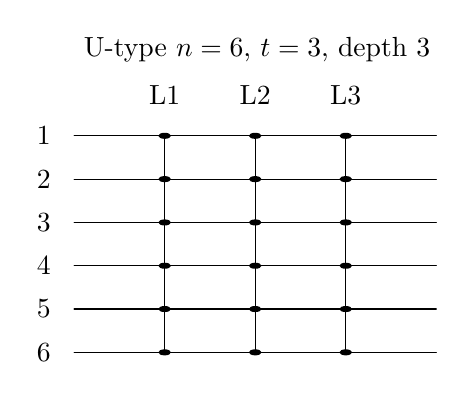
\begin{tikzpicture}[x=1.15cm,y=0.55cm,line cap=round]
  \node[anchor=west] at (0,1) {U-type $n=6$, $t=3$, depth 3};
  \draw (0,-1) -- (4,-1);
  \node[anchor=east] at (-0.15,-1) {1};
  \draw (0,-2) -- (4,-2);
  \node[anchor=east] at (-0.15,-2) {2};
  \draw (0,-3) -- (4,-3);
  \node[anchor=east] at (-0.15,-3) {3};
  \draw (0,-4) -- (4,-4);
  \node[anchor=east] at (-0.15,-4) {4};
  \draw (0,-5) -- (4,-5);
  \node[anchor=east] at (-0.15,-5) {5};
  \draw (0,-6) -- (4,-6);
  \node[anchor=east] at (-0.15,-6) {6};
  \node[anchor=south] at (1,-0.5) {L1};
  \draw (1,-1) -- (1,-3);
  \fill (1,-1) circle (0.07);
  \fill (1,-3) circle (0.07);
  \draw (1,-2) -- (1,-6);
  \fill (1,-2) circle (0.07);
  \fill (1,-6) circle (0.07);
  \draw (1,-4) -- (1,-5);
  \fill (1,-4) circle (0.07);
  \fill (1,-5) circle (0.07);
  \node[anchor=south] at (2,-0.5) {L2};
  \draw (2,-1) -- (2,-5);
  \fill (2,-1) circle (0.07);
  \fill (2,-5) circle (0.07);
  \draw (2,-2) -- (2,-3);
  \fill (2,-2) circle (0.07);
  \fill (2,-3) circle (0.07);
  \draw (2,-4) -- (2,-6);
  \fill (2,-4) circle (0.07);
  \fill (2,-6) circle (0.07);
  \node[anchor=south] at (3,-0.5) {L3};
  \draw (3,-1) -- (3,-6);
  \fill (3,-1) circle (0.07);
  \fill (3,-6) circle (0.07);
  \draw (3,-2) -- (3,-5);
  \fill (3,-2) circle (0.07);
  \fill (3,-5) circle (0.07);
  \draw (3,-3) -- (3,-4);
  \fill (3,-3) circle (0.07);
  \fill (3,-4) circle (0.07);
\end{tikzpicture}
